\section{Zeitauswertung}

\subsection{Zweck dieses Dokuments}
Die Zeitauswertung zeigt auf, wann und wo wieviel Zeit aufgewendet wurde. Dabei haben wir drei unterschiedliche Auswertungen angefertigt, welche in den nachfolgenden Unterkapitel genauer erläutert werden.

\subsection{Zeitliche Auswertung nach Monaten}
Die erste Auswertung zeit die aufgewendete Zeit nach Monaten. 
Über die vier Monate, in denen das Projekt lief, wurden insgesamt 477 Stunden aufgewendet. Dies entspricht ziemlich genau dem Richtwert von 480 Stunden. 
Da das Projekt am 17. September 2018 startete, fallen die 80 Stunden, welche im September eingesetzt wurden, geringer aus als in den restlichen Monaten. In den Monaten Oktober und November wurden ca. 140 Stunden bzw. 150 Stunden investiert. Im Dezember gingen die aufgewendeten Stunden auf 102 zurück.

\begin{figure}[h]
  \centering
  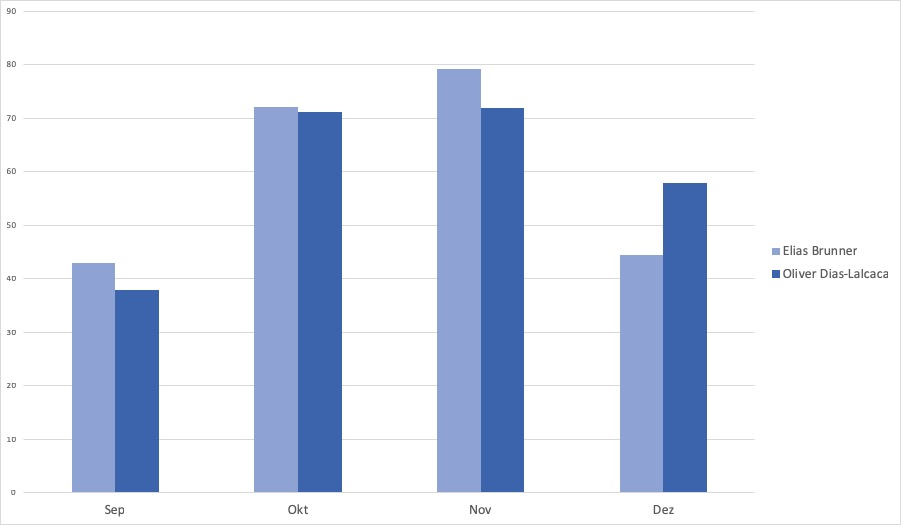
\includegraphics[width=1\linewidth]{./img/zeitauswertung/ZeitauswertungMonate}
  \caption{Zeitliche Auswertung nach Monaten}
  \label{fig:comparison-month}
\end{figure}

\subsection{Zeitliche Auswertung nach Sprints}
Sieht man sich die Zeitauswertung anhand der durchgeführten Sprints an, fällt auf, dass in den ersten drei Sprints vermeintlich sehr viel Zeit gebucht wurde. So ist zum Beispiel der Sprint \grqq Elaboration-2\grqq{} mit einem gesamten Stundenaufwand von 115 Stunden zu verbuchen wobei in \grqq Construction-4\grqq{} etwas mehr als 4 Stunden aufgewendet worden sein sollen.

Dieses Verhalten resultiert daraus, dass Jira die gesamte Zeit auf jenen Sprint bucht, in welcher das Ticket erstellt wurde. Da gerade zu Beginn eines Projektes mehr Tickets erstellt werden (auch haben wir viele Tickets über mehrere Sprints hinweg bearbeitet) als gegen Ende, ergibt sich diese Verteilung.
 
Die Auswertung nach Sprints ist daher mit Vorsicht zu verstehen.

\begin{figure}[h]
  \centering
  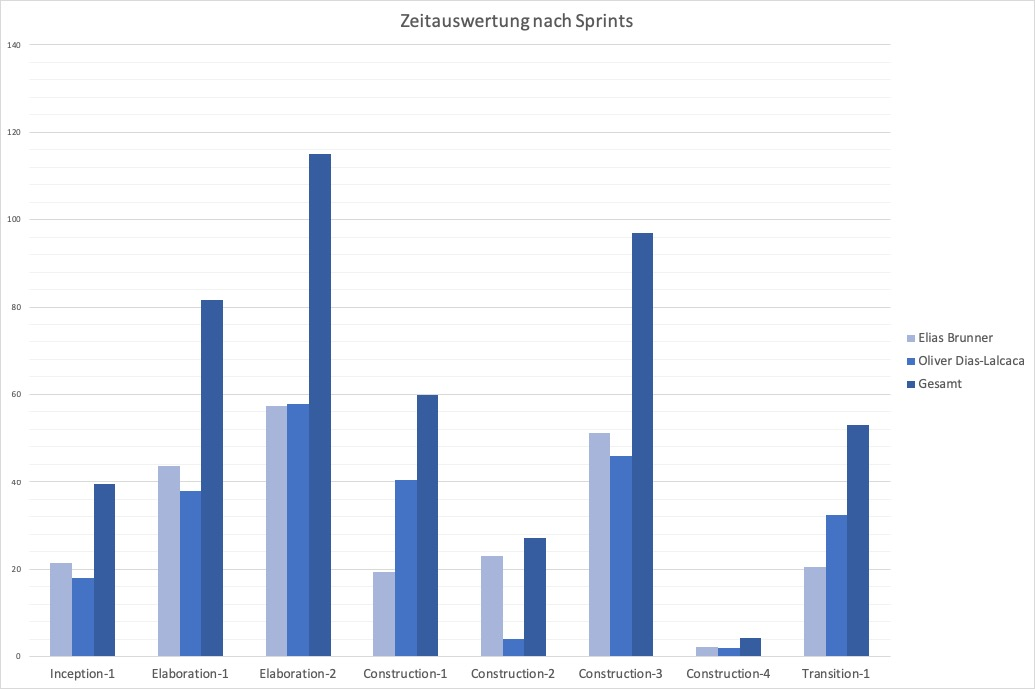
\includegraphics[width=1\linewidth]{./img/zeitauswertung/ZeitauswertungSprints}
  \caption{Zeitliche Auswertung nach Sprints}
  \label{fig:comparison-sprints}
\end{figure}

\subsection{Zeitliche Auswertung nach Arbeitskategorien}
Zuletzt interessierte uns noch wie viel Zeit wir für die einzelnen Arbeitskategorien (Labels) aufgewendet haben. Hierbei ist anzumerken, dass wir einem Ticket teilweise mehr als eine Arbeitskategorie zugewiesen haben, was dazu führt, dass die aufgeschriebene Zeit für jede zugewiesene Arbeitskategorie summiert wird.

Die prozentuale Aussage gibt dennoch ein ungefähren Überblick über die investierten Zeiten für die einzelnen Arbeitskategorien.

Um das Diagramm zu verstehen muss gesagt werden, dass der innerste Kreis die Zeiten für Elias Brunner repräsentieren, der mittlere Kreis die Zeiten für Oliver Dias-Lalcaca und der äusserste Kreis den Mittelwert der Beiden darstellt.

\begin{figure}
	\centering
	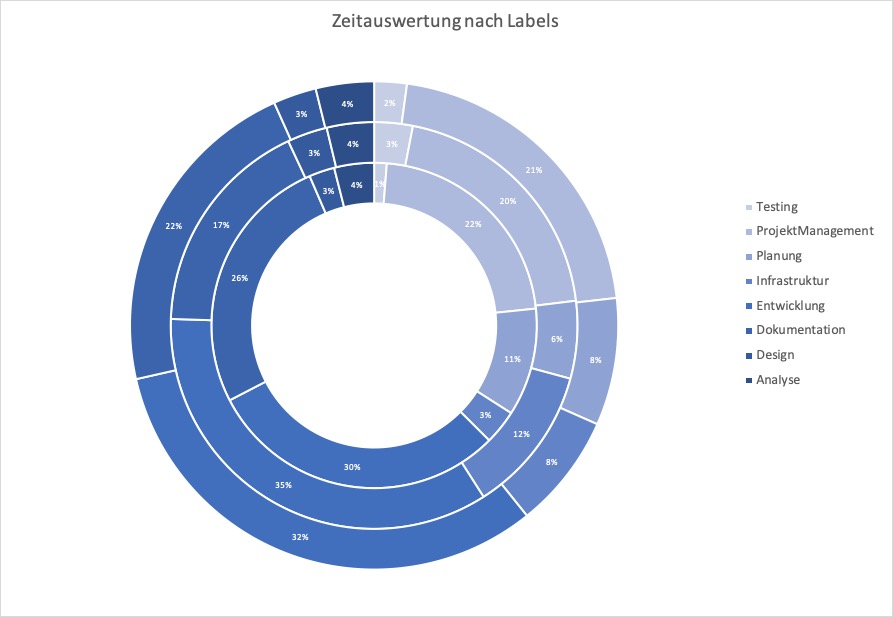
\includegraphics[width=1\linewidth]{./img/zeitauswertung/ZeitauswertungLabel}
	\caption{Zeitliche Auswertung nach Labels}
	\label{fig:comparison-labels}
\end{figure}